\documentclass[12pt]{article}
\usepackage[margin=1 in]{geometry}
\usepackage{graphicx}
\usepackage{float}
\usepackage{booktabs}
\usepackage{siunitx}
\usepackage{amsmath}
\usepackage{amssymb}

\title{Lab 10: LTSpice Analysis of Active Filters}
\author{Sean Balbale}
\date{November 11th, 2024}
\setlength{\parindent}{0in}

\begin{document}

\begin{titlepage}
  \begin{center}
    \vspace*{1in}

    \Huge
    \textbf{Lab 10}

    \LARGE
    LTSpice Analysis of Active Filters

    \vspace{3 in}

    \textbf{Student Name:} Sean Balbale
    \\ \textbf{Instructor:} Dr. Iman Salama
    \\ \textbf{Lab Partner Name:} Krish Gupta
    \\ \textbf{Date:} November 15, 2024

    \vfill

  \end{center}
\end{titlepage}

\newpage

\section{Introduction}
Operational amplifiers (op-amps) have served as essential components in
electronic circuit design, particularly in sensing and signal processing
applications. This lab focused on constructing active filters with op-amps,
which are critical for biomedical applications such as electrocardiogram (EKG)
signal measurement. These filters were designed to amplify small signals while
selectively filtering out noise, thereby enhancing signal quality by rejecting
common-mode interference and removing unwanted frequency components. Through
LTSpice simulations, low-pass and high-pass filter designs were examined to
analyze their frequency responses, cutoff frequencies, and time-domain
performance. This approach provided insights into the role of active filters in
real-world signal processing, forming a foundation for practical applications in
biomedical and other electronic systems.

\section{Results}
% \begin{figure}[H]
%   \centering
%   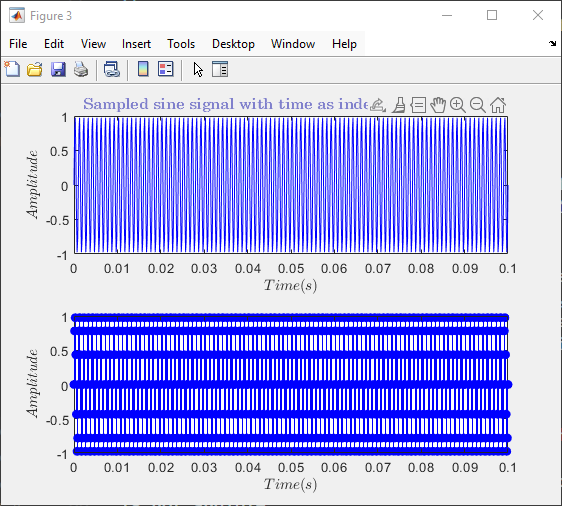
\includegraphics[width=0.3\textwidth]{fig 1f 7000.png}\hfill
%   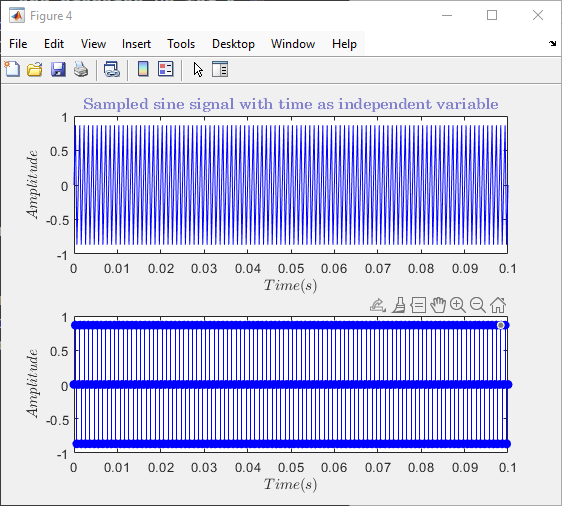
\includegraphics[width=0.3\textwidth]{fig 1f 3000.png}\hfill
%   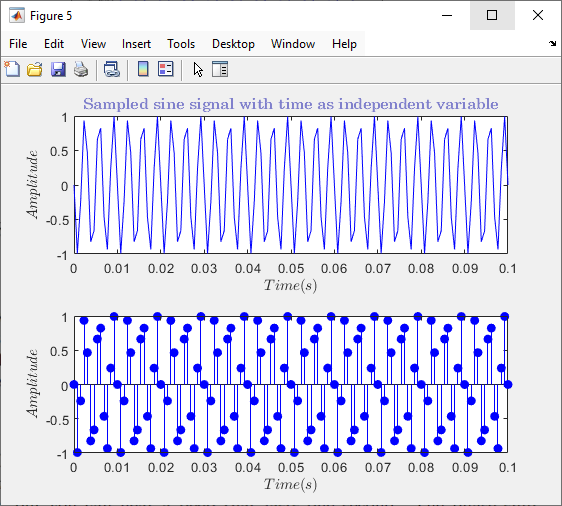
\includegraphics[width=0.3\textwidth]{fig 1f 1300.png}
%   \caption{Sinusoidal with $f_s$ = 7 kHz, 3 kHz, and 1.3 kHz}
%   \label{fig:fig3}
% % \end{figure}

\subsection{LTSpice Modeling of Op Amp Circuits}
\subsubsection{Low Pass Filters}
\begin{figure}[H]
  \centering
  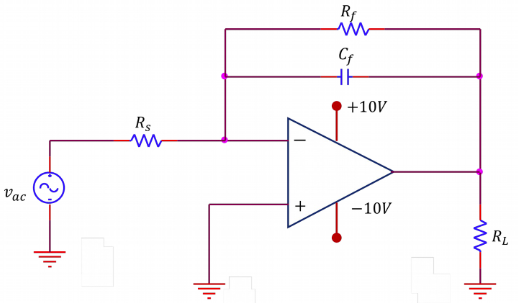
\includegraphics[width=0.5\textwidth]{photos/First Order Active Low Pass Filter.png}
  \caption{First Order Active Low Pass Filter}
  \label{fig:FirstOrderActiveLowPassFilter}
\end{figure}

A first order low pass filter was constructed using an op-amp, resistors
($R_f$, $R_s$, $R_L$), and capacitor ($C_f$). Following the circuit design
(Figure \ref{fig:FirstOrderActiveLowPassFilter}), the circuit was simulated in LTSpice
with $\pm \SI{10}{\volt} \; DC$ power supplies, $R_f = \SI{100}{\kilo\ohm}$, $R_s = \SI{20}{\kilo\ohm}$,
$R_L = \SI{1}{\kilo\ohm}$, and $C_f = \SI{10}{\nano\farad}$. The voltage input was a
AC input with a $\SI{0.1}{\volt}$ amplitude and a frequency sweep from $\SI{1}{\hertz}$
to $\SI{1}{\mega\hertz}$.
\newline

The frequency cutoff can be calculated using the formula:
\[
  \begin{aligned}
    f_c & = \frac{1}{2\pi R_f C_f}                                         \\
    & = \frac{1}{2\pi \times 100 \times 10^3 \times 10 \times 10^{-9}} \\
    & = \SI{159.1}{\hertz}
  \end{aligned}
\]

This results in a cutoff frequency of $\SI{159.1}{\hertz}$.

This value is what is expected to be seen since there is a time constant of
$\SI{1}{\milli\second}$. Which was calculated using the formula:
\[
  \begin{aligned}
    \tau & = R_f \times C_f \\
    & = 100 \times 10^3 \times 10 \times 10^{-9} \\
    & = \SI{1}{\milli\second}
  \end{aligned}
\]
These theoretical values are confirmed by the LTSpice simulation results shown in Figure \ref{fig:1.2Results}.
\begin{figure}[H]
  \centering
  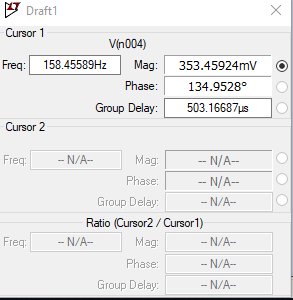
\includegraphics[width=0.5\textwidth]{Lab 10 Shared/1.2 simulation results.PNG}
  \caption{LTSpice Simulation Results}
  \label{fig:1.2Results}
\end{figure}

\begin{figure}[H]
  \centering
  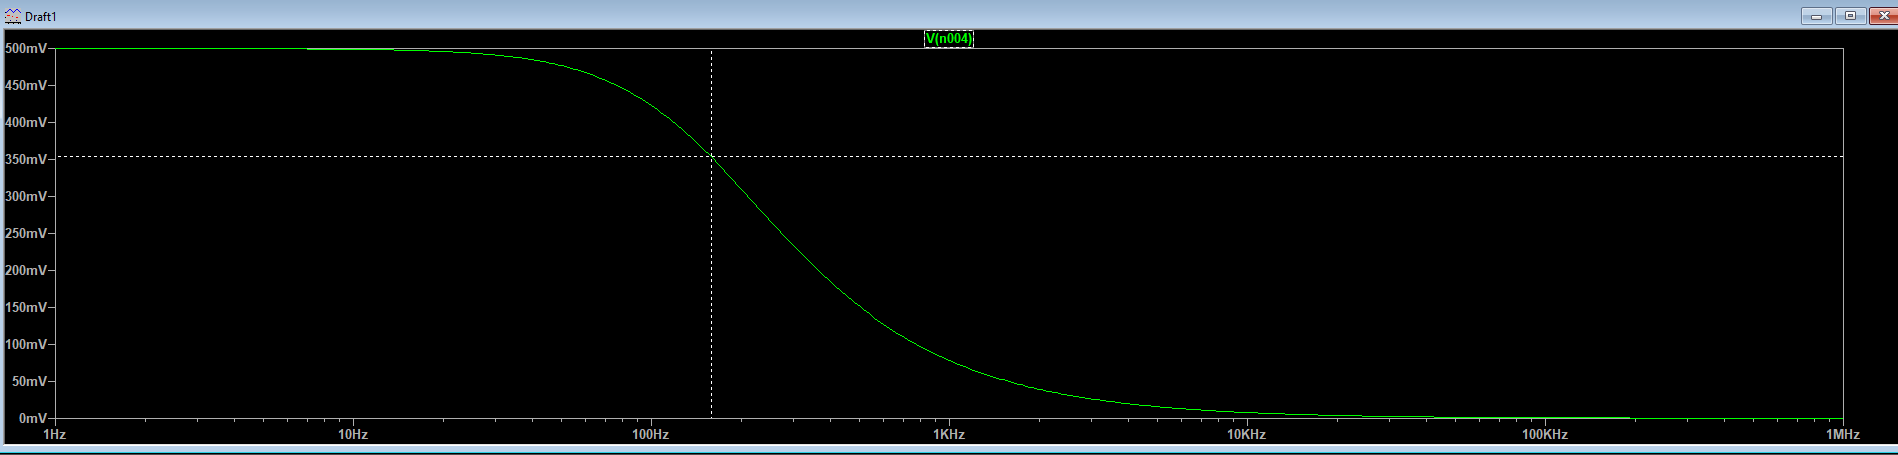
\includegraphics[width=1\textwidth]{Lab 10 Shared/1.2 simulation.PNG}
  \caption{LTSpice Simulation}
  \label{fig:1.2Simulation}
\end{figure}
These results can also be calculated by hand from Figure \ref{fig:1.2Simulation}.
Next, the amplitude of the input sinusoid was increased to $\SI{0.5}{\volt}$.
The simulation is shown in Figure \ref{fig:1.3Simulation} and
the results are shown in Figure \ref{fig:1.3Results}.
\begin{figure}[H]
  \centering
  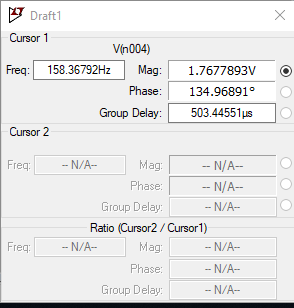
\includegraphics[width=0.5\textwidth]{Lab 10 Shared/1.3 simulation results.PNG}
  \caption{LTSpice Simulation Results}
  \label{fig:1.3Results}
\end{figure}

\begin{figure}[H]
  \centering
  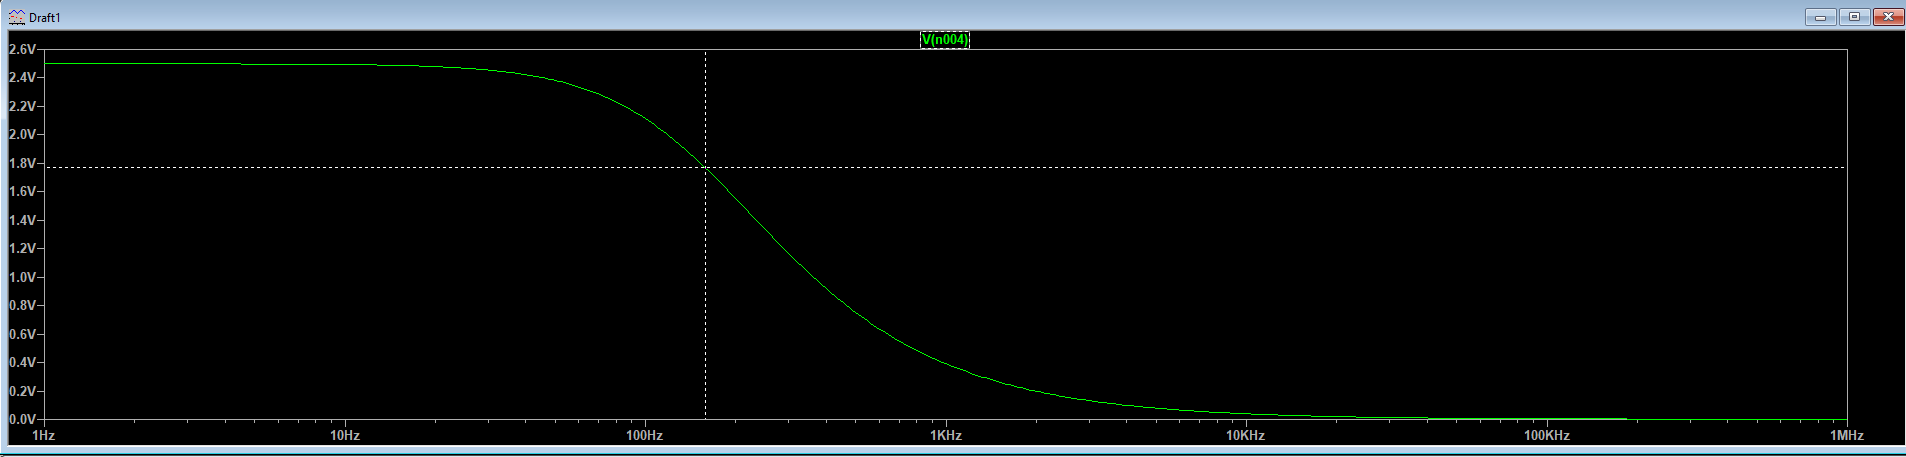
\includegraphics[width=1\textwidth]{Lab 10 Shared/1.3 simulation.PNG}
  \caption{LTSpice Simulation}
  \label{fig:1.3Simulation}
\end{figure}

The frequency cuttoff and time constant are the same as
the previous simulation. This should have been clear from the
formulas for the cutoff frequency and time constant. The amplitude
of the input sinusoid was increased to $\SI{0.5}{\volt}$, but the
cutoff frequency and time constant are not dependent on the amplitude.
\newline

\begin{figure}[H]
  \centering
  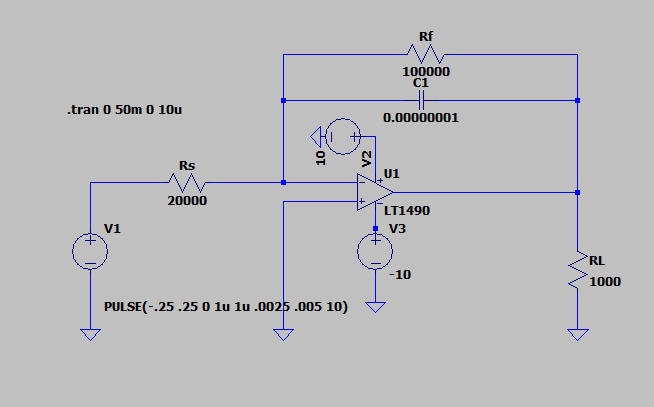
\includegraphics[width=0.5\textwidth]{Lab 10 Shared/1.4 circuit.PNG}
  \caption{LTSpice Circuit}
  \label{fig:1.4Circuit}
\end{figure}
A new circuit was constructed for a first order high pass filter.
The circuit is shown in Figure \ref{fig:1.4Circuit}. The input and output
voltages were probed and the simulation was run. The results are shown in
Figure \ref{fig:1.4Results}.
\begin{figure}[H]
  \centering
  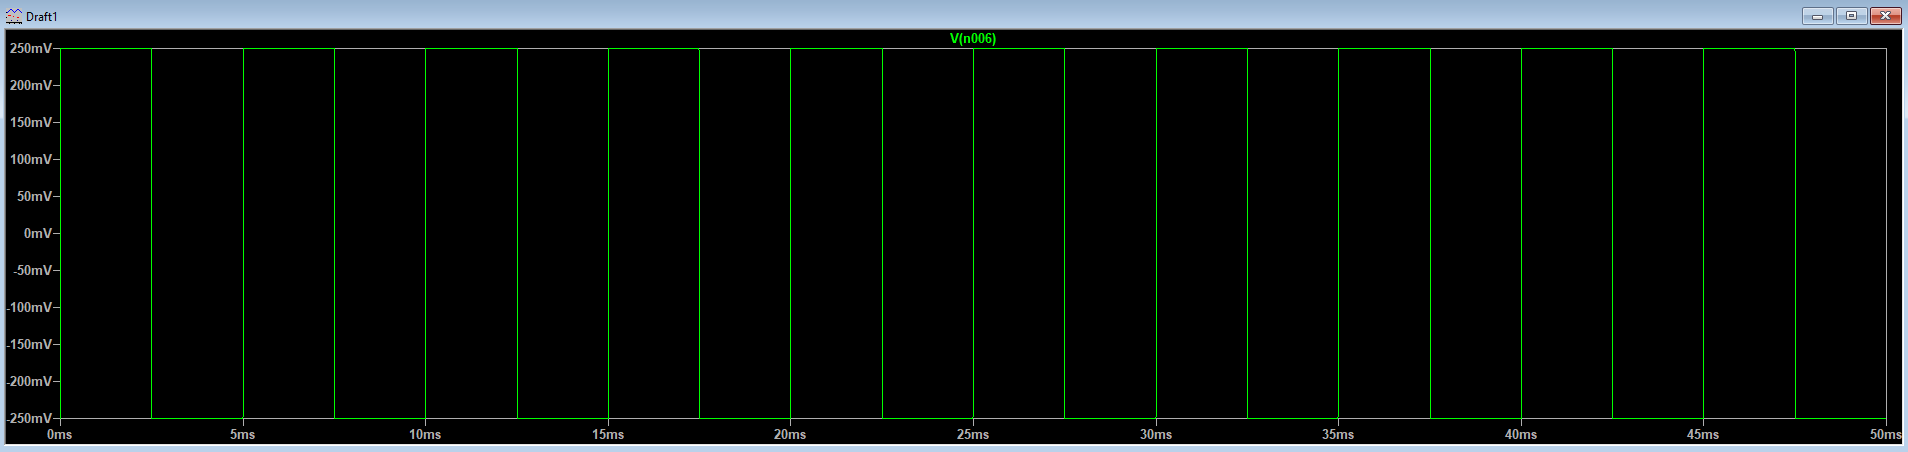
\includegraphics[width=1\textwidth]{Lab 10 Shared/1.4 input simulation.PNG} \\
  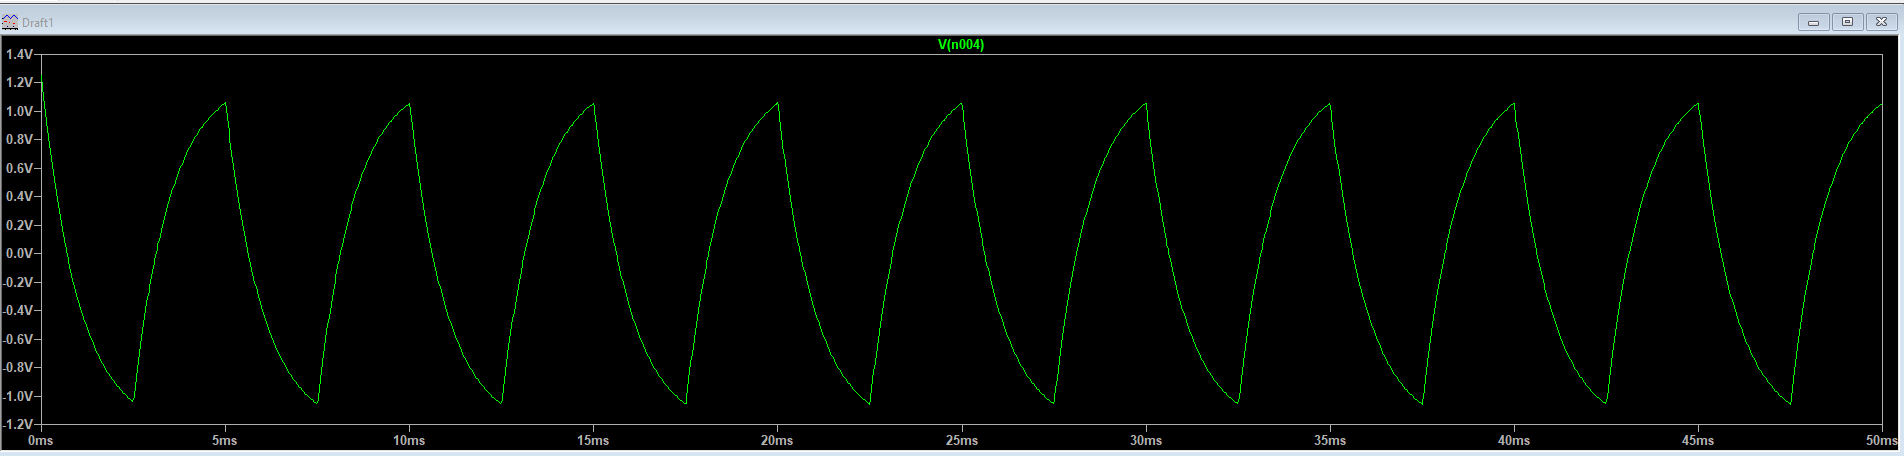
\includegraphics[width=1\textwidth]{Lab 10 Shared/1.4 output simulation.PNG}
  \caption{LTSpice Input (Top) and Output (Bottom) Simulation Results}
  \label{fig:1.4Results}
\end{figure}
The input is a regular square wave. The output is also a square wave but
the capacitor is charging and discharging. This results in more of a point
at the top of a logarhythmic curve.

\subsubsection{High Pass Filters}
Now a first order high pass filter was constructed using an op-amp, resistors
($R_f$, $R_s$, $R_L$), and capacitor ($C_f$). Following the circuit design
(Figure \ref{fig:FirstOrderActiveHighPassFilter}), the circuit was simulated in LTSpice (Figure \ref{fig:1.5Circuit}).
\begin{figure}[H]
  \centering
  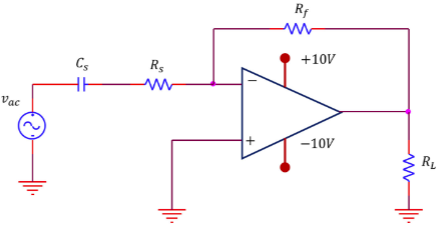
\includegraphics[width=0.5\textwidth]{photos/First Order Active High Pass Filter.png}
  \caption{First Order High Pass Filter Circuit}
  \label{fig:FirstOrderActiveHighPassFilter}
\end{figure}

The circuit was simulated with $\pm \SI{10}{\volt} \; DC$ power supplies,
$R_f = \SI{200}{\kilo\ohm}$, $R_s = \SI{100}{\kilo\ohm}$, $C_s = \SI{10}{\nano\farad}$.
The voltage input was a AC input with a $\SI{0.1}{\volt}$ amplitude and a frequency sweep from $\SI{1}{\hertz}$
to $\SI{1}{\mega\hertz}$.

\begin{figure}[H]
  \centering
  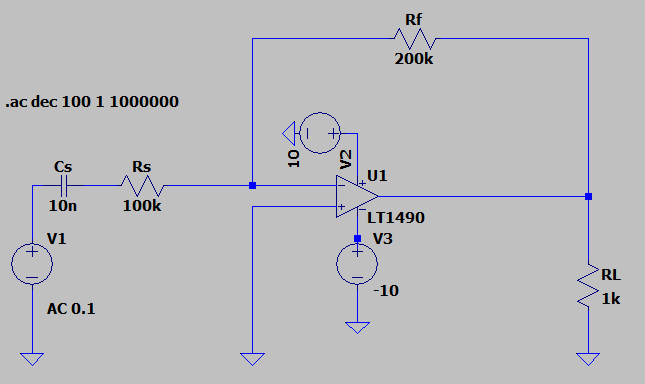
\includegraphics[width=0.5\textwidth]{Lab 10 Shared/1.5 circuit.PNG}
  \caption{LTSpice Circuit}
  \label{fig:1.5Circuit}
\end{figure}

The frequency cutoff can be calculated using the formula:
\[
  \begin{aligned}
	f_c & = \frac{1}{2\pi R_s C_f}                                         \\
	& = \frac{1}{2\pi \times 100 \times 10^3 \times 10 \times 10^{-9}} \\
	& = \SI{159.1}{\hertz}
  \end{aligned}
\]

The in-band gain can be calculated using the formula:
\[
  \begin{aligned}
	Gain & = -\frac{R_f}{R_s} \\
	& = -\frac{200 \times 10^3}{100 \times 10^3} \\
	& = -2
  \end{aligned}
\]

The simulation is shown in Figure \ref{fig:1.5Simulation} and
the results are shown in Figure \ref{fig:1.5Results}. These results
support the theoretical calculations for the cutoff frequency.
\begin{figure}[H]
  \centering
  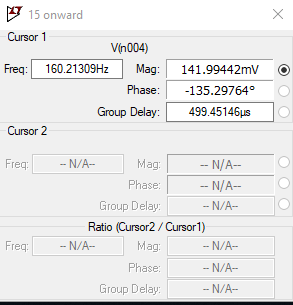
\includegraphics[width=0.5\textwidth]{Lab 10 Shared/1.5 simulation results.PNG}
  \caption{LTSpice Simulation Results}
  \label{fig:1.5Results}
\end{figure}

\begin{figure}[H]
  \centering
  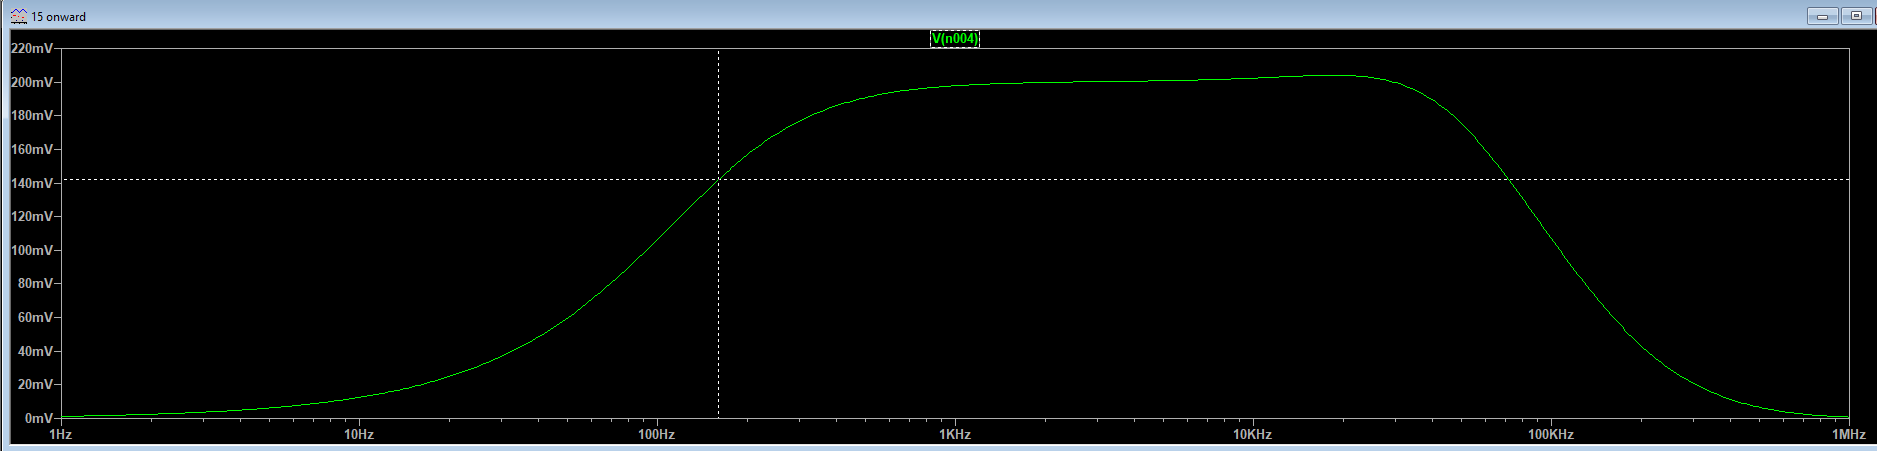
\includegraphics[width=1\textwidth]{Lab 10 Shared/1.5 simulation.PNG}
  \caption{LTSpice Simulation}
  \label{fig:1.5Simulation}
\end{figure}

In the simulation, the output rolls off at higher frequencies. This behavior 
can be seen in Figure \ref{fig:1.5Simulation}. This occurs because the input
frequency exceeds the maximum op-amp frequency. This results in the avalanche
effect seen in the graph.


\section{Discussion and Conclusion}
This lab successfully demonstrated the design and analysis of active low-pass
and high-pass filters using LTSpice. The simulations confirmed theoretical
predictions for cutoff frequencies and gain, and the filters performed as
expected in both frequency and time domains. The low-pass filter effectively
attenuated high frequencies, with a confirmed cutoff frequency of $\SI{159.
1}{\hertz}$, while the high-pass filter attenuated low frequencies with a
matching cutoff. Additionally, the observed roll-off at high frequencies in the
high-pass filter simulation illustrated the op-amp’s bandwidth limitations, a
crucial consideration in real-world filter applications.
\newline

Through these exercises, this lab highlighted the critical role of component
selection in filter design, the effect of op-amp bandwidth on filter performance,
and the practical applications of active filters in biomedical signal
processing. Overall, the experiment reinforced the value of LTSpice as a
simulation tool and provided foundational insights for implementing filters in
various signal processing applications.


\section{References}
[1] Dr. Iman Salama. “Lab 10 – LTSpice Analysis of Active Filters” Northeastern University. 11 November 2024.

\end{document}
